\documentclass[10pt,landscape,twocolumn,letterpaper,twosided]{article}

\usepackage{hyperref}
\usepackage[spanish, activeacute]{babel}
\usepackage[utf8]{inputenc}
\usepackage{fancyhdr}
\usepackage{lastpage}
\usepackage{listings}
\usepackage{amssymb}
\usepackage[usenames,dvipsnames]{color}
\usepackage{graphicx}
\usepackage{wrapfig}
\usepackage{amsmath}
\usepackage{makeidx}
\usepackage{verbatim}
\usepackage{color}
\usepackage{geometry}
\usepackage{multicol}
\usepackage{multirow}
\usepackage{supertabular}
\usepackage{booktabs}
\usepackage{float}
\geometry{verbose,landscape,letterpaper,tmargin=2cm,bmargin=2cm,lmargin=1.5cm,rmargin=1.5cm}


%%%%%%%%%%%%%%%%%%%%%importar codigo desde archivos cpp
\lstloadlanguages{C++}
\lstnewenvironment{code}
	{%\lstset{	numbers=none, frame=lines, basicstyle=\small\ttfamily, }%
	 \csname lst@SetFirstLabel\endcsname}
	{\csname lst@SaveFirstLabel\endcsname}
\lstset{% general command to set parameter(s)
	language=C++, basicstyle=\small\ttfamily, keywordstyle=\slshape,
	emph=[1]{tipo,usa}, emphstyle={[1]\sffamily\bfseries},
	morekeywords={tint,forn,forsn},
	basewidth={0.47em,0.40em},
	columns=fixed, fontadjust, resetmargins, xrightmargin=5pt, xleftmargin=15pt,
	flexiblecolumns=false, tabsize=2, breaklines,	breakatwhitespace=false, extendedchars=true,
	numbers=left, numberstyle=\tiny, stepnumber=1, numbersep=9pt,
	frame=l, framesep=3pt,
    basicstyle=\ttfamily,
    keywordstyle=\color{blue}\ttfamily,
    stringstyle=\color{magenta}\ttfamily,
    commentstyle=\color{RedOrange}\ttfamily,
    morecomment=[l][\color{OliveGreen}]{\#}
}

\lstdefinestyle{C++}{
	language=C++, basicstyle=\small\ttfamily, keywordstyle=\slshape,
	emph=[1]{tipo,usa,tipo2}, emphstyle={[1]\sffamily\bfseries},
	morekeywords={tint,forn,forsn},
	basewidth={0.47em,0.40em},
	columns=fixed, fontadjust, resetmargins, xrightmargin=5pt, xleftmargin=15pt,
	flexiblecolumns=false, tabsize=2, breaklines,	breakatwhitespace=false, extendedchars=true,
	numbers=left, numberstyle=\tiny, stepnumber=1, numbersep=9pt,
	frame=l, framesep=3pt,
    basicstyle=\ttfamily,
    keywordstyle=\color{blue}\ttfamily,
    stringstyle=\color{magenta}\ttfamily,
    commentstyle=\color{RedOrange}\ttfamily,
    morecomment=[l][\color{OliveGreen}]{\#}
}

%%% Macros
\def\nbtitle#1{\begin{Large}\begin{center}\textbf{#1}\end{center}\end{Large}}
\def\nbsection#1{\section{#1}}
\def\nbsubsection#1{\subsection{#1}}
\def\nbcoment#1{\begin{small}\textbf{#1}\end{small}}
\newcommand{\comb}[2]{\left( \begin{array}{c} #1 \\ #2 \end{array}\right)}
\def\complexity#1{\texorpdfstring{$\mathcal{O}(#1)$}{O(#1)}}
 \newcommand\cppfile[2][]{
\lstinputlisting[style=C++,linerange={#1}]{#2}
}

\setlength{\columnsep}{0.25in}

\begin{document}
	
	\title{Repositorio en C++}
	\author{Universidad de la Amazonia, Colombia.}
	\maketitle
	
	\begin{center}
		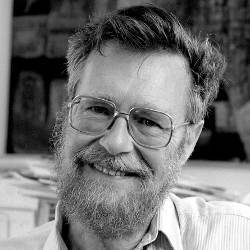
\includegraphics[scale=0.9]{dijkstra}
		\Huge{I2}
	\end{center}
	\normalsize
	\tableofcontents
	\hfill
	
		\section{Estructuras de datos}
			\subsection{Tablas aditivas}
			Construcción O(n), Consulta O(1)
			\cppfile[16-33]{estructuras_de_datos/tablas_aditivas.cpp}
			\subsection{Disjoint set union find}
			Asocia elementos en conjuntos de arboles.\\
			Construcción O(n)
			\cppfile[7-44]{estructuras_de_datos/disjoint_set_union_find.cpp}
			%\subsection{Union find con compresion de caminos}
			%Asocia elementos de manera simple.
			%\cppfile[9-22]{estructuras_de_datos/union_find-compresion_de_caminos.cpp}
			\subsection{Segment tree}
			Ejemplo de RMQ (Range Minium Query)\\
			Construcción O(n), Consulta O(log n), Update O(log n)
			\cppfile[8-68]{estructuras_de_datos/segment_tree.cpp}%29-84
			\subsection{Segment tree con lazy propagation}
			Permite actualizar rangos del árbol en O(log n).\\
			solo están los métodos nuevos y los que hay que actualizar, lo demás es lo mismo del segment tree normal.
			\cppfile[29-84]{estructuras_de_datos/segment_tree_lazy_propagation.cpp}
			\subsection{Arbol de Fenwick}
			Estructura para el RSM(Range Sum Query)\\
			Construcción O(n log n), Consulta O(log k), Update O(log n)
			\cppfile[8-35]{estructuras_de_datos/arbol_binario_indexado.cpp}
			\subsection{Sparse table}
			Para RMQ (Range Minium Query) en arreglos estaticos\\
			Construcción O(n log n), Consulta O(1)
			\cppfile[8-35]{estructuras_de_datos/Sparse_table.cpp}
			\subsection{Set extendido}
			Set indexado.
			\cppfile[2-10]{estructuras_de_datos/set_extendido.cpp}
			
		\section{Grafos}
			\subsection{Dijkstra}
			Ruta minima
			O((n + m)log n)
			\cppfile[12-46]{grafos/dijkstra.cpp}
			\subsection{Bellman-Ford}
			Ruta minima con pesos negativos
			O($n^{2}$)
			\cppfile[12-33]{grafos/bellman-Ford.cpp}
			\subsection{Floyd Warshall}
			Ruta minima de toda una matriz de adyacencia, recomendable si n $\leq$ 100\\	
			O($n^{3}$)
			\cppfile[8-36]{grafos/floyd.cpp}
			\subsection{kosaraju}
			Componentes fuertemente conexas grafos si y no dirigidos\\
			O(2(n + m))
			\cppfile[9-36]{grafos/kosaraju.cpp}
			\subsection{Tarjan}
			Componentes fuertemente conexas grafos si y no dirigidos, requiere menos
			espacio que kosaraju\\
			O(n + m)
			\cppfile[9-39]{grafos/tarjan.cpp}
			\subsection{Kruskal}
			Arbol generador minimo(MST) usando lista de aristas, se necesita de un union-find.
			O(m log n), sin contar el ordenamiento.
			\cppfile[38-57]{grafos/kruskal.cpp}
			\subsection{Prim}
			Arbol generador minimo (MST)\\
			O(m log n)
			\cppfile[10-34]{grafos/prim.cpp}
			\subsection{Topological sort}%%%ORDENAMIENTO TOPOLOGICO
			O(n + m), algoritmo de kahn.
			\cppfile[7-26]{grafos/topological_sort_para_grafos_ciclicos.cpp}
			\subsection{Puntos de articulación y puentes}
			O(n + m).
			\cppfile[10-48]{grafos/puntos_de_articulacion_y_puentes.cpp}
			\subsection{Maximum flow}%%maximo flujo
			Flujo maximo en un grafo. Algoritmo de Edmonds Karp O(${VE}^{2}$)
			\cppfile[12-53]{grafos/Edmonds_karp.cpp}
			\subsection{Min cost Max flow}
			Flujo maximo manteniendo minimo costo.
			\cppfile[6-59]{grafos/min_cost_max_flow.cpp}
			\subsection{Ruta minima en un DAG}
			O(V+2E)
			\cppfile[12-44]{grafos/ruta_minima_DAG.cpp}
			\subsection{Tour de Euler}
			\cppfile[10-33]{grafos/tour_euleriano.cpp}
			\subsection{Lowest Common Ancestor}
			Ancestro común mas bajo en un arbol, para u y v encontrar el nodo mas bajo que este por encima de
			ambos.\\
			Solucion con Range Minimum Query (sparse table).
			\cppfile[38-65]{otros/Lowest_Common_Ancestor.cpp}
			Solucion con construcción O(n log n) y consultas O(log n)
			\cppfile[11-77]{otros/Lowest_Common_Ancestor_logN.cpp}
			\subsection{Conectividad dinámica}
			\cppfile[7-70]{grafos/conectividad_dinamica.cpp}			
			
		\section{Programacion dinamica}
			\subsection{Subconjuntos de un conjunto}
			O($2^{n}$)
			\cppfile[6-15]{programacion_dinamica/bitmask.cpp}
			\subsection{Problema de la mochila}
			\cppfile[8-23]{programacion_dinamica/knapsack.cpp}
			\subsection{Longest Increment Subsecuence}
			Subsecuencia creciente mas larga, solución corta con dp\\
			O((n*(n+1))/2)
			\cppfile[48-57]{programacion_dinamica/longest_increasing_subsequence.cpp}
			Solución D{\&}C con gredy, O(n log n)
			\cppfile[7-46]{programacion_dinamica/longest_increasing_subsequence.cpp}
			\subsection{Max Range Sum}
			Algoritmo de Kadane, O(n)
			\cppfile[6-22]{programacion_dinamica/Max_Range_Sum.cpp}
			\subsection{Subset Sum}
			\cppfile[8-20]{programacion_dinamica/Subset_Sum.cpp}
			\subsection{Traveling salesman problem}
			O($2^{n}*n^{2}$), para la respuesta llamar: tsp(0,1)
			\cppfile[7-22]{programacion_dinamica/traveling_salesman_problem.cpp}
		
		\section{Otros}
			\subsection{Busqueda binaria}
			O(log n)
			\cppfile[7-19]{otros/busqueda_binaria.cpp}
			\subsection{Raiz babilonica}
			Encuentra la raiz cuadrada de un numero
			\cppfile[4-12]{otros/raiz_babilonica.cpp}
			\subsection{Codigo gray}
			\cppfile[5-12]{otros/codigo_gray.cpp}
			\subsection{Método de Wilson}
			Encuentra n! mod p, con p primo, requiere el inverso modular
			\cppfile[23-30]{otros/teorema_wilson.cpp}
			
		\section{Matematicas}
			\subsection{MCD y MCM}
			Maximo comun divisor(MCD) y minimo comun multiplo(MCM)
			\cppfile[5-6]{matematicas/MCD_y_MCM.cpp}
			\subsection{Phi de euler}
			Devuelve la cantidad de coprimos de un numero n, complejidad O($\sqrt{n}$) 
			\cppfile[5-14]{matematicas/phi_de_euler.cpp}
			\subsection{Algoritmo extendido de euclides}
			Encuentra dos numeros x e y tal que: MCD(a, b) = ax + by
			\cppfile[5-15]{matematicas/algoritmo_extendido_de_euclides.cpp}
			\subsection{Ecuaciones diofanticas}
			Resuelve ecuaciones de la forma aX+bY=c
			\cppfile[20-38]{matematicas/ecuaciones_diofanticas.cpp}
			\subsection{Exponenciacion binaria}
			O(log n)
			\cppfile[6-13]{matematicas/exponenciacion_binaria.cpp}
			\subsection{Multiplicacion modular}
			Encuentra (a*b) mod c, la operacion puede generar overflow
				si se realiza directamente, el metodo mulmod evita el overflow usando un
				ciclo, pero se puede usar el tipo de dato int128 de c++11 para poder calcular
				de manera directa, pero el int128 no se puede leer o imprimir directamente.
			\cppfile[5-26]{matematicas/multiplicacion_modular.cpp}
			\subsection{Exponenciacion modular}
			Encuentra $(a^b)$ mod c, se nesecita implementar previamente multiplicacion modular.
			\cppfile[16-20]{matematicas/exp_modular.cpp}
			\subsection{Inverso modular}
			Encontrar $x$ talque $a*x \equiv 1\% m$, el primer método requiere algoritmo extendido de euclides y el 
			segundo exponenciacion modular
			\cppfile[34-43]{matematicas/inverso_multiplicativo_modular.cpp}
			\subsection{Logaritmo discreto}
			Encuentra una solución para $a^{x} \equiv 1 (mod(p))$.\\ O($\sqrt{m} log (m)$)
			\cppfile[7-25]{matematicas/logaritmo_discreto.cpp}
			\subsection{Test de Rabin Miller}
			Devuelve si un numero es primo, requiere de implementar previamente GCD(maximo común divisor),
			multiplicacion modular y exponenciacion modular.
			\cppfile[27-50]{matematicas/test_de_rabin_miller.cpp}
			\subsection{Rho de pollard}
			Factorizacion rapida, usar para $n > 10^{12}$ , requiere de implementar previamente el GCD
			(maximo común divisor), multiplicacion modular,	exponenciacion modular y el test de Rabin Miller.\\
			O($\sqrt[4]{n}$)
			\cppfile[52-77]{matematicas/rho_de_pollard.cpp}
			\subsection{Factorizacion con criba}
			Factorizacion usando la criba, usar para $n \leq 10^{12}$, guarda los factores en un mapa 
			similar a rho de pollard.
			\cppfile[10-48]{matematicas/factorizacion_criba.cpp}
			\subsection{Divisores}
			Encontrar los divisores de un numero según su factorización
			\cppfile[82-100]{matematicas/divisores.cpp}
			%\subsection{BigInteger c++}
			%\cppfile[4-197]{matematicas/biginteger.cpp}
			\subsection{Fraccion}
			\cppfile[9-45]{matematicas/fraccion.cpp}
			\subsection{Matrices}
			Exponenciación de matrices: $M^b$ en O($n^{3} log (b)$)
			\cppfile[8-36]{matematicas/matrices.cpp}
			\subsection{FFT}
			Multiplicación rápida de polinomios y enteros, complejidad O(n*log(n))
			\cppfile[10-67]{matematicas/FFT.cpp}
		\section{Cadenas}
			\subsection{Algoritmo de bordes}
			Encuentra la longitud del mayor borde de un string n.
			\cppfile[4-16]{cadenas/bordes.cpp}
			\subsection{KMP}
			Encuentra si una cadena n es subcadena de otra cadena m, requiere de implementar
			y ejecutar previamente el algoritmo de bordes\\
			O(n+m)
			\cppfile[18-29]{cadenas/kmp.cpp}
			\subsection{Tablas hash}
			\cppfile[7-19]{cadenas/Hashing.cpp}
			\subsection{String alignment}
			Mínima distancia entre dos string.\\O(s1*s2)
			\cppfile[8-25]{cadenas/string_distance.cpp}
			\subsection{Arreglo de sufijos}
			\cppfile[7-48]{cadenas/Arreglo_de_sufijos.cpp}
			\subsection{Longest common prefix}
			Requiere implementar arreglo de sufijos.
			\cppfile[50-65]{cadenas/Arreglo_de_sufijos.cpp}
			\subsection{String matching}
			Requiere implementar arreglo de sufijos con la cadena principal.
			\cppfile[92-114]{cadenas/Arreglo_de_sufijos.cpp}
			\subsection{Subcadena común mas larga}
			Requiere implementar arreglo de sufijos y Longest common prefix.
			\cppfile[67-90]{cadenas/Arreglo_de_sufijos.cpp}
			
		\section{Geometria}
			\subsection{Punto}
			\cppfile[22-59]{geometria/punto.cpp}
			\subsection{Linea y segmento}
			Linea de la forma $ax + by + c = 0$.
			\cppfile[42-105]{geometria/linea.cpp}
			\subsection{Vector}
			\cppfile[39-66]{geometria/vector.cpp}
			\subsection{Convex Hull}
			Polígono convexo con perímetro mínimo que cubre todos los puntos, verificar que no hallan puntos 
			repetidos, O(n log n)
			\cppfile[48-79]{geometria/convex_hull.cpp}
			\subsection{Área de un polígono}
			Área de un polígono, resultado con coordenadas en sentido horario: positivo, anti-horario: negativo, 
			y cero si están desordenados, O(n)
			\cppfile[59-67]{geometria/poligono.cpp}
			\subsection{Punto en poligono}
			Verifica si un punto esta dentro de un polígono, O(n)
			\cppfile[80-104]{geometria/poligono.cpp}
			\subsection{Minimum covering circle}
			Mínimo circulo que puede cubrir todos los puntos
			\cppfile[20-60]{geometria/minimum_covering_circle.cpp}
			\subsection{Nearest pair of points}
			Mínima distancia entre dos puntos O(n)
			\cppfile[18-67]{geometria/nearestPairPoints.cpp}
	
	%Basado en el notebook C++ de la UFPS 2017
	\section{Formulas}

		\subsection{Tabla ASCII}
			Caracteres ASCII con sus respectivos valores numéricos.
%		\begin{center}
		\begin{table}[H]
			\begin{tabular}{|l|l|l|l|l|l|l|l|}
				\hline \textbf{No.} & \textbf{ASCII} & \textbf{No.} & \textbf{ASCII}  &
					\textbf{No.} & \textbf{ASCII} & \textbf{No.} & \textbf{ASCII} \\ \hline
				32 & space & 40 & ( & 48 & 0 & 56 & 8 \\ \hline
				33 &  ! & 41 & ) & 49 & 1 & 57 & 9 \\ \hline
				34 &  " & 42 & * & 50 & 2 & 58 & : \\ \hline
				35 & \# & 43 & + & 51 & 3 & 59 & ; \\ \hline
				36 & \$ & 44 & , & 52 & 4 & 60 & < \\ \hline
				37 & \% & 45 & - & 53 & 5 & 61 & = \\ \hline
				38 & \& & 46 & . & 54 & 6 & 62 & > \\ \hline
				39 &  ' & 47 & / & 55 & 7 & 63 & ? \\ \hline
			\end{tabular}
		\end{table}
		
		
%		\begin{table}[H]
			\begin{tabular}{|l|l|l|l|l|l|l|l|}
				\hline \textbf{No.} & \textbf{ASCII} & \textbf{No.} & \textbf{ASCII}  &
					\textbf{No.} & \textbf{ASCII} & \textbf{No.} & \textbf{ASCII} \\ \hline
				64 & @ & 72 & H & 80 & P & 88 & X \\ \hline
				65 & A & 73 & I & 81 & Q & 89 & Y \\ \hline
				66 & B & 74 & J & 82 & R & 90 & Z \\ \hline
				67 & C & 75 & K & 83 & S & 91 & [ \\ \hline
				68 & D & 76 & L & 84 & T & 92 & \textbackslash \\ \hline
				69 & E & 77 & M & 85 & U & 93 & ] \\ \hline
				70 & F & 78 & N & 86 & V & 94 & \textasciicircum \\ \hline
				71 & G & 79 & O & 87 & W & 95 & \_ \\ \hline
			\end{tabular}
%		\end{table}
		
%		\begin{table}[H]
			\begin{tabular}{|l|l|l|l|l|l|l|l|}
				\hline \textbf{No.} & \textbf{ASCII} & \textbf{No.} & \textbf{ASCII}  &
					\textbf{No.} & \textbf{ASCII} & \textbf{No.} & \textbf{ASCII} \\ \hline
				96 & ` & 104 & h & 112 & p & 120 & x \\ \hline
				97 & a & 105 & i & 113 & q & 121 & y \\ \hline
				98 & b & 106 & j & 114 & r & 122 & z \\ \hline
				99 & c & 107 & k & 115 & s & 123 & \{ \\ \hline
				100 & d & 108 & l & 116 & t & 124 & \textbar \\ \hline
				101 & e & 109 & m & 117 & u & 125 & \} \\ \hline
				102 & f & 110 & n & 118 & v & 126 & \textasciitilde \\ \hline
				103 & g &  111 & o & 119 & w & 127 &  \\ \hline
			\end{tabular}
%		\end{table}
%		\end{center}
		
		%\newpage


\subsection{Formulas generales}

%\begin{center}
%\tablefirsthead{}
%\tabletail{
%	\midrule 
%}
%\tablelasttail{}
%{\renewcommand{\arraystretch}{1.4}


%\begin{table}[H]
\begin{tabular}{|p{6.5cm}|p{3.9cm}|}
	\hline
	\multicolumn{2}{|c|}{PERMUTACIÓN Y COMBINACIÓN} \\ \hline
	Combinación (Coeficiente Binomial): Número de subconjuntos de k elementos escogidos de un conjunto con n elementos.
		& $ \binom{n}{k} = \binom{n}{n-k} = \displaystyle\frac{n!}{k!(n-k)!} $ \\ \hline

	Combinación con repetición: Número de grupos formados por n elementos, partiendo de m tipos de elementos.
		& $ \binom{m+n-1}{n} = \displaystyle\frac{(m + n - 1)!}{n!(m-1)!} $ \\ \hline
		
	Permutación: Número de formas de agrupar n elementos, donde importa el orden y sin repetir elementos
		& $ P_{n} = n! $ \\ \hline

	Permutación múltiple: Elegir r elementos de n posibles con repetición 
		& $ n^{r} $	\\ \hline
	
	Permutación con repetición: Se tienen n elementos donde el primero se repite a veces, el segundo b veces, etc.
		& $ PR_{n}^{a,b,c...} = \displaystyle\frac{P_{n}}{a!b!c!...}$ \\ \hline
	
	Permutaciones sin repetición: Número de formas de agrupar r elementos de n disponibles, sin repetir elementos
		& $\displaystyle\frac{n!}{(n-r)!}$ \\ \hline
\end{tabular}
%\end{table}


\begin{tabular}{|p{2.2cm}|p{8.2cm}|}
	\hline
	\multicolumn{2}{|c|}{DISTANCIAS} \\ \hline
	Distancia Euclideana & $d_{E}(P_{1},P_{2}) = \sqrt{(x_{2}-x_{1})^{2}+(y_{2}-y_{1})^{2}}$ \\ \hline
	Distancia Manhattan & $d_{M}(P_{1}, P_{2}) = |x_{2} - x_{1}| + |y_{2} - y_{1}|$ \\ \hline 
\end{tabular}

\begin{tabular}{|p{2.0cm}|p{2.8cm}|p{2.0cm}|p{2.8cm}|}
	\hline
	\multicolumn{4}{|c|}{CIRCUNFERENCIA Y CÍRCULO} \\  \hline
	\multicolumn{4}{|p{10cm}|}{Considerando $r$ como el radio, $\alpha$ como el ángulo del arco o sector, y (R, r) 
		como radio mayor y menor respectivamente.} \\ \hline
	Área                   & $A = \pi * r^{2} $ & Longitud & $L = 2*\pi*r$  \\ \hline
	Longitud de un arco    & $L = \displaystyle\frac{2*\pi*r*\alpha}{360}$ & Área sector circular 
		& $A = \displaystyle\frac{\pi * r^{2} * \alpha}{360}$ \\ \hline
	Área corona circular   & $A = \pi  (R^{2} - r^{2})$ & Formula general & $(X-P_{x})^{2}+(Y-P_{y})^2=r^{2}$ \\ \hline 
\end{tabular}

\begin{tabular}{|p{2.0cm}|p{2.8cm}|p{2.0cm}|p{2.8cm}|}
	\hline
	\multicolumn{4}{|c|}{TRIÁNGULO} \\  \hline

	\multicolumn{4}{|p{10cm}|}{Considerando $b$ como la longitud de la base, $h$ como la altura, letras minúsculas 
	como la longitud de los lados, letras mayúsculas como los ángulos, y $r$ como el radio de círcunferencias 
	asociadas.} \\ \hline
	
	Área con base y altura & $A = \displaystyle\frac{1}{2}b * h$ &
		Área con 2 lados y su ángulo & $A = \displaystyle\frac{1}{2}b*a*sin(C)$ \\ \hline
	Área con los 3 lados & \multicolumn{3}{ |c|} {$ A = \sqrt{p(p - a)(p - b)(p - c)}$ con 
		$p = \displaystyle\frac{a + b + c}{2}$ } \\ \hline
	Triángulo circunscrito a circunferencia & $A = \displaystyle\frac{abc}{4r}$ &
		Triángulo inscrito a circunferencia & $A = r(\displaystyle\frac{a+b+c}{2})$ \\ \hline
	Triangulo equilátero & $A = \displaystyle\frac{\sqrt{3}}{4}a^{2}$ & & \\ \hline 
\end{tabular}

\begin{tabular}{|p{3.3cm}|p{3.3cm}|p{3.3cm}|}
	\hline
	\multicolumn{3}{|c|}{TRIGONOMÉTRIA} \\ \hline
	
	$sin(\alpha) = \displaystyle\frac{opuesto}{hipotenusa}$ 
		& $cos(\alpha) = \displaystyle\frac{adyacente}{hipotenusa}$
		& $tan(\alpha) = \displaystyle\frac{opuesto}{adyacente}$ \\ \hline
		
	$sec(\alpha) = \displaystyle\frac{1}{cos(\alpha)}$ 
		& $csc(\alpha) = \displaystyle\frac{1}{sin(\alpha)}$
		& $cot(\alpha) = \displaystyle\frac{1}{tan(\alpha)}$ \\ \hline
	
	Ley de los senos, con $\gamma$ el angulo opuesto al lado $c$ & \multicolumn{2}{ |c|} {$\displaystyle\frac{a}{sin(\alpha)} 
		= \frac{b}{sin(\beta)} = \frac{c}{sin(\gamma)}$ } \\ \hline
	Ley de los cosenos, con $\gamma$ el angulo opuesto al lado $c$ & \multicolumn{2}{ |c|} {$ c^{2} = 
		a^{2}+b^{2}-2ab*cos(\gamma)$ } \\ \hline
	
\end{tabular}

\begin{tabular}{|p{2.2cm}|p{8.2cm}|}
	\hline
	\multicolumn{2}{|c|}{PROPIEDADES DEL MÓDULO (RESIDUO)} \\  \hline
	Neutra & (a \% b) \% b = a \% b \\ \hline
	Asociativa en suma & (a + b) \% c = ((a \% c) + (b \% c)) \% c \\ \hline
	Asociativa en multiplicación &  (a*b) \% c = ((a \% c)*(b \% c)) \% c \\ \hline
\end{tabular}

\begin{tabular}{|p{2.2cm}|p{8.2cm}|}
	\hline
	\multicolumn{2}{|c|}{CONSTANTES} \\ \hline
	Pi & $\pi = acos(-1) \approx 3.14159$ \\ \hline
	e & $e \approx 2.71828$ \\ \hline
	Número áureo & $\phi = \displaystyle\frac{1 + \sqrt{5}}{2} \approx 1.61803$  \\ \hline
\end{tabular}

\begin{tabular}{|p{2.0cm}|p{2.8cm}|p{2.0cm}|p{2.8cm}|}
	\hline
	\multicolumn{4}{|c|}{FIGURAS} \\ \hline
	Elipse & $A = PI*a*b $ & Cono & $ V = \frac{1}{3} * PI*r^{2}*h$ \\ \hline
	Cilindro & $V = PI*r^{2}*h$ & Esfera & $V = \frac{4}{3}*PI*r^{3}$  \\ \hline
\end{tabular}

%}
%\end{center}


\subsection{Sequences}
Listado de secuencias mas comunes y como hallarlas.

\begin{center}
\tablefirsthead{}
\tabletail{
\midrule 
\multicolumn{2}{r}{{Continúa en la siguiente columna}} \\}
\tablelasttail{}
{\renewcommand{\arraystretch}{1.4}
\begin{supertabular}{|p{1.8cm}|p{8.6cm}|}

\hline

\multirow{2}{2cm}{Estrellas octangulares}
& 	0, 1, 14, 51, 124, 245, 426, 679, 1016, 1449, 1990, 2651, ...
\\ \cline{2-2}
& $f(n) = n*(2*n^{2} - 1)$.
\\ \hline

\multirow{2}{2cm}
{Euler totient}    
& 1, 1, 2, 2, 4, 2, 6, 4, 6, 4, 10, 4, 12, 6,...            
\\ \cline{2-2} 
& $f(n) = $ Cantidad de números $\leq n$ coprimos con n. 
\\ \hline

\multirow{2}{2cm}{Números de Bell} 
& 1, 1, 2, 5, 15, 52, 203, 877, 4140, 21147, 115975, ...
\\ \cline{2-2} 
& Se inicia una matriz triangular con f[0][0] = f[1][0] = 1. La suma de estos dos se guarda en f[1][1] y se traslada a f[2][0]. Ahora se suman f[1][0] con f[2][0] y se guarda en f[2][1]. Luego se suman f[1][1] con f[2][1] y se guarda en f[2][2] trasladandose a f[3][0] y así sucesivamente. Los valores de la primera columna contienen la respuesta.
\\ \hline

\multirow{2}{2cm}
{Números de Catalán} 
& 1, 1, 2, 5, 14, 42, 132, 429, 1430, 4862, 16796, 58786, ...
\\ \cline{2-2}
& $f(n)=\displaystyle\frac{(2n)!}{(n + 1)! n!}$
\\ \hline

\multirow{2}{2cm}{Números de Fermat}
& 3, 5, 17, 257, 65537, 4294967297, 18446744073709551617, ...
\\ \cline{2-2}
& $f(n) = 2^{(\displaystyle2^{\textstyle n})} + 1$
\\ \hline

\multirow{2}{2cm}
{Números de Lucas} 
& 2, 1, 3, 4, 7, 11, 18, 29, 47, 76, 123, 199, 322, ...    
\\ \cline{2-2} 
& $f(0) = 2$; $f(1) = 1$; $f(n) = f(n-1) + f(n-2)$ para $n>1$            
\\ \hline

\multirow{2}{2cm}{Números de Pell} 
& 0, 1, 2, 5, 12, 29, 70, 169, 408, 985, 2378, 5741, 13860, ...
\\ \cline{2-2} 
& $f(0) = 0; f(1) = 1; f(n) = 2f(n-1) + f(n-2)$ para $n>1$
\\ \hline

\multirow{2}{2cm}
{Números de Tribonacci} 
& 0, 0, 1, 1, 2, 4, 7, 13, 24, 44, 81, 149, 274, 504, ...    
\\ \cline{2-2} 
& $f(0)=f(1)=0; f(2)=1; f(n) = f(n-1) + f(n-2) + f(n-3)$ para $n>2$
\\ \hline

\multirow{2}{2cm}{Números piramidales cuadrados}
& 0, 1, 5, 14, 30, 55, 91, 140, 204, 285, 385, 506, 650, ...
\\ \cline{2-2}
& $f(n) = \displaystyle\frac{n*(n+1)*(2*n+1)}{6}$
\\ \hline

\multirow{2}{2cm}{Números primos de Mersenne}
& 3, 7, 31, 127, 8191, 131071, 524287, 2147483647, ...
\\ \cline{2-2}
& $f(n) = 2^{p(n)} - 1$ donde $p$ representa valores primos iniciando en $p(0)=2$.
\\ \hline

\multirow{2}{2cm}{Números tetraedrales}
& 0, 1, 4, 10, 20, 35, 56, 84, 120, 165, 220, 286, 364, ...
\\ \cline{2-2}
& $f(n) = \displaystyle\frac{n*(n+1)*(n+2)}{6}$
\\ \hline

\multirow{2}{2cm}{Números triangulares}
& 0, 1, 3, 6, 10, 15, 21, 28, 36, 45, 55, 66, 78, 91, 105, ...
\\ \cline{2-2}
& $f(n) = \displaystyle\frac{n(n+1)}{2}$
\\ \hline

\multirow{2}{2cm}{OEIS A000127}
& 1, 2, 4, 8, 16, 31, 57, 99, 163, 256, 386, 562, ...
\\ \cline{2-2}
& $f(n) = \displaystyle\frac{(n^{4}-6n^{3}+23n^{2}-18{n}+24)}{24}$.
\\ \hline

\multirow{2}{2cm}{Secuencia de Narayana}
& 1, 1, 1, 2, 3, 4, 6, 9, 13, 19, 28, 41, 60, 88, 129, ...
\\ \cline{2-2}
& $f(0) = f(1) = f(2) = 1; f(n) = f(n-1) + f(n-3)$ para todo $n>2$.
\\ \hline

\multirow{2}{2cm}
{Secuencia de Silvestre} 
& 2, 3, 7, 43, 1807, 3263443, 10650056950807, ...    
\\ \cline{2-2} 
& $f(0) = 2; f(n+1) = f(n)^2 - f(n) + 1$               
\\ \hline

\multirow{2}{2cm}{Secuencia de vendedor perezoso} 
& 1, 2, 4, 7, 11, 16, 22, 29, 37, 46, 56, 67, 79, 92, 106, ...
\\ \cline{2-2} 
& Equivale al triangular(n) + 1. Máxima número de piezas que se pueden formar al hacer n cortes a un disco. 

$f(n) = \displaystyle\frac{n(n+1)}{2} + 1$
\\ \hline

\multirow{2}{2cm}{Suma de los divisores de un número}
& 1, 3, 4, 7, 6, 12, 8, 15, 13, 18, 12, 28, 14, 24, ...
\\ \cline{2-2}
&Para todo $n>1$ cuya descomposición en factores primos es $n=\displaystyle p_{1}^{\textstyle a_{1}}\displaystyle p_{2}^{\textstyle a_{2}}...\displaystyle p_{k}^{\textstyle a_{k}}$ se tiene que:

$f(n) = \displaystyle\frac{p_{1}^{a_{1} + 1} - 1}{p_{1} - 1} * \frac{p_{2}^{a_{2} + 1} - 1}{p_{2} - 1} * ... * \frac{p_{k}^{a_{k} + 1} - 1}{p_{k} - 1}$ 
\\ \hline

\multirow{2}{2cm}{Schroeder numbers} 
& 1, 1, 3, 11, 45, 197, 903, 4279, 20793, 103049, 518859, ...
\\ \cline{2-2} 
& El número de formas de insertar paréntesis en una secuencia y el número de formas de partir un polígono convexo en polígonos más pequeños mediante la inserción de diagonales. f(1)=f(2)=1;

$f(n) = \displaystyle\frac{3(2n-3)*f(n-1) - (n-3)*f(n-2)}{n}$
\\ \hline

\end{supertabular}
}
\end{center}
\subsection{Time Complexities}

Aproximación del mayor número n de datos que pueden procesarse para cada una de las complejidades algoritmicas. Tomar esta tabla solo como referencia.

\begin{tabbing}
\textbf{Complexity}\hspace{4cm} \=  \textbf{n}\hspace{3cm}   \\ 
$O(n!)$ \> 11\\ 
$O(2^{n}*n^{2})$ \> 18\\ 
$O(2^{n}*n)$ \> 22\\ 
$O(n^{4})$ \> 100\\ 
$O(n^{3})$ \> 500\\ 
$O(n^{2}\log_{2}n)$ \> 1.000\\ 
$O(n^{2})$ \> 10.000\\ 
$O(n\log_{2}n)$ \> $10^{6}$\\ 
$O(n)$ \> $10^{8}$\\ 
$O(\sqrt{n})$ \> $10^{16}$\\ 
$O(\log_{2}n)$ \> -\\ 
$O(1)$ \> -\\ 
\end{tabbing}



	\section{Extras}
		\subsection{Template}
			Plantilla de typedef, define, etc.
			\cppfile[1-29]{otros/template.cpp}
		
		\subsection{Ayudas}
			\cppfile[34-62]{otros/template.cpp}
		
		%\newpage
		\subsection{Formulas extra}
			
			\begin{center}
				\tablefirsthead{}
				\tabletail{
				\midrule 
				\multicolumn{2}{r}{{Continúa en la siguiente columna}} \\}
				\tablelasttail{}
				{\renewcommand{\arraystretch}{1.4}
				\begin{supertabular}{|p{2.2cm}|p{8.2cm}|}
					\hline
					\multicolumn{2}{|c|}{} \\
					\multicolumn{2}{|c|}{Formulas extras} \\
					\multicolumn{2}{|c|}{} \\ \hline
					
					Formula de números fibonacci &
					
					\vspace{1mm}
					{\Large $f(n) = \frac{1}{\sqrt{5}} * [ (\frac{1 + \sqrt{5}}{2})^{n}  - 
						(\frac{1 - \sqrt{5}}{2})^{n}]$ }
					\\ \hline
					
					Ecuación de la recta que pasa por dos puntos & y = mx + b.
					
					{\Large $\frac{x - x_{1}}{x_{2} - x_{1}} = \frac{y - y_{1}}{y_{2} - y_{1}}$}
					\\ \hline
					
					Ecuación del plano que pasa por 3 puntos & Al resolver la determinante, se tiene el plano que 
					pasa por 3 puntos de la forma (x,y,z).
					
					$\begin{vmatrix}
						X-x_{1} &Y-y_{1} &Z-z_{1} \\ 
						x_{2}-x_{1} &y_{2}-y_{1} &z_{2}-z_{1} \\ 
						x_{3}-x_{1} &y_{3}-y_{1} &z_{3}-z_{1}
					\end{vmatrix} = 0$
					\\ \hline
					
					Distancia de un punto a una recta & Teniendo una recta con formula de la forma: $ax + by + c$ 
					la distancia mínima a un punto p de la forma $(px, py)$ la distancia minima esta dada por la 
					formula.
					
					{\Large $d = \frac{a*px + b*py + c}{\sqrt{a^{2} + b^{2}}}$}
					\\ \hline
					
					Formula de triángulos degenerados & Si el resultado es mayor a 0.5 es un triángulo de calidad 
					buena. Es posible formar un triangulo si $a+b>c$ con $c>b>a$.
					
					{\Large $\frac{(a + b - c) * (a + c - b) * (b  + c - a)} {a * b * c}$}				
					\\ \hline

					Formula de fibonacci con matrices &
					
					{\large
					$\begin{bmatrix}
						1 & 1\\ 
						1 & 0
					\end{bmatrix}^{b} =
					\begin{bmatrix}
						fib(b+1) & fib(b) \\ 
						fib(b) & fib(b-1)
					\end{bmatrix}$}
					\\ \hline
					
					Progresión aritmética & Sea $d$ la diferencia y $a_{1}$ el numero inicial, entonces $a_{n} = 
					a_{1}+(n-1)d$. y la sumatoria de los primeros n elementos es:
					
					\vspace{1mm}
					{\Large$\sum_{i=1}^{n}a_{i} = n\frac{a_{1}+a_{n}}{2}$}
					\\ \hline
					
					Progresión geométrica & Sea $r$ la razón y $a_{1}$ el numero inicial, entonces $a_{n} = 
					a_{1}*r^{n-1}$ y la sumatoria de los primeros n elementos es:
					
					{\large
					$\sum_{i=1}^{n}a_{i} = a_{1} * \frac{r^{n}-1}{r-1}$}
					\\ \hline
					
					Teorema de Erd\H{o}s–Gallai & Una secuencia de enteros $d_{1} \geq ... \geq d_{n}$ puede 
					representar una secuencia de grados de un grafo si y solo si: para cada k en $1 \leq k \leq n$
					
					{\large
					$\sum_{i=1}^{k} d_{i} \leq k(k+1)+\sum_{i=k+1}^{n} min(d_{i},k)$}
					\\ \hline
					
					Cantidad de divisores de un numero & con n = $p_{1}^{a_{1}}*p_{2}^{a_{2}}*...*p_{k}^{a_{k}}$ 
					la cantidad sera:
					
					{\Large$\prod_{i=1}^{k} a_{i}+1$}
					\\ \hline
					
					Coeficientes binomiales & Encuentra $n$ combinado $k$. para construir el triangulo de pascal 
					solo poner en $n$ la fila y en $k$ la columna.
					
					$C(n, k) = 	
					\begin{cases}
						0 & \text{k=0,n=k}\\
						C(n-1,k-1)+C(n-1,k) & \text{c.c.}
					\end{cases}
					$
					\\ \hline
					
					Números de catalán & Encontrar numero de arboles binarios de n nodos, numero 
					de formas de emparejar paréntesis.
					
					{\large
					$Cat(n) = 	
					\begin{cases}
						1 & \text{si $n = 0$}\\
						\frac{2n*(2n-1) * Cat(n-1)}{(n+1)*n} & \text{c.c.}
					\end{cases}
					$}
					\\ \hline
					
					Teorema de Pick & Sea $A$ el área de un polígono con puntos enteros, $B$ la cantidad de puntos 
					enteros en el borde, $I$ la cantidad de puntos enteros interiores, entonces:
					
					$A = I + \frac{B}{2} - 1$
					\vspace{1mm}
					\\ \hline
					
					%Determinante de Gauss & Encontrar el área de un polígono en el plano cartesiano a partir de 
					%sus vértices.
					%{\large$A = \frac{1}{2} $}
					%{\large $ \begin{bmatrix}
					%	x_{1} & y_{1} \\ 
					%	x_{2} & y_{2} \\ 
					%	x_{n} & y_{n} \\ 
					%	x_{1} & y_{1} 
					%\end{bmatrix}$ }
					%\vspace{1mm}
					%{\large $S = x_{1}y_{2} + x_{2}y_{3} +...+ x_{n}y_{1}$}
					%\vspace{1mm}
					%{\large $D = x_{2}y_{1} + x_{3}y_{2} +...+ x_{1}y_{n}$} 
					%\vspace{1mm}
					%{\large $A = \frac{1}{2} |S - D|$}
					%\\ \hline
					
					%Agregar:
					%a^phi(n) es congruente con 1 mod n
					%los divisores de phi(x) son posibles soluciones para a^x congruente con 1 mod m
				\end{supertabular}
				}
			\end{center}

			
		\subsection{Secuencias}
		
		\textbf{Primos:}\\
		\vspace{3mm}
			2 3 5 7 11 13 17 19 23 29 31 37 41 43 47 53 59 61 67 71 73 79 83 89 97 101 103 107 109 113 127 131 137 139
			149 151 157 163 167 173 179 181 191 193 197 199 211 223 227 229 233 239 241 251 257 263 269 271 277 281 283
			293 307 311 313 317 331 337 347 349 353 359 367 373 379 383 389 397 401 409 419 421 431 433 439 443 449 457
			461 463 467 479 487 491 499 503 509 521 523 541 547 557 563 569 571 577 587 593 599 601 607 613 617 619 631
			641 643 647 653 659 661 673 677 683 691 701 709 719 727 733 739 743 751 757 761 769 773 787 797 809 811 821
			823 827 829 839 853
			857 859 863 877 881 883 887 907 911 919 929 937 941 947 953 967 971 977 983 991 997 1009 1013 1019 1021 1031
			1033 1039 1049 1051 1061 1063 1069 1087 1091 1093 1097 1103 1109 1117 1123 1129 1151 1153 1163 1171 1181 1187
			1193 1201 1213 1217 1223 1229 1231 1237 1249 1259 1277 1279 1283 1289 1291 1297 1301 1303 1307 1319 1321 1327
			1361 1367 1373 1381 1399 1409 1423 1427 1429 1433 1439 1447 1451 1453 1459 1471 1481 1483 1487 1489 1493 1499
			1511 1523 1531 1543 1549 1553 1559 1567 1571 1579 1583 1597 1601 1607 1609 1613 1619 1621 1627 1637 1657 1663
			1667 1669 1693 1697 1699 1709 1721 1723 1733 1741 1747 1753 1759 1777 1783 1787 1789 1801 1811 1823 1831 1847
			1861 1867 1871 1873 1877 1879 1889 1901 1907 1913 1931 1933 1949 1951 1973 1979 1987 1993 1997 1999 2003 2011
			2017 2027 2029 2039 2053 2063 2069 2081 2083 2087 2089 2099 2111 2113 2129 2131 2137 2141 2143 2153 2161 2179
			2203 2207 2213 2221 2237 2239 2243 2251 2267 2269 2273 2281 2287 2293 2297 2309 2311 2333 2339 2341 2347 2351
			2357 2371 2377 2381 2383 2389 2393 2399 2411 2417 2423 2437 2441 2447 2459 2467 2473 2477

	\vspace{8mm}
	\textbf{Primos cercanos a potencias de 10:}\\
	\vspace{3mm}
	7 11, 89 97 101 103, 983 991 997 1009 1013 1019, 
	9941 9949 9967 9973 10007 10009 10037 10039 10061 10067 10069 10079, 
	99961 99971 99989 99991 100003 100019 100043 100049 100057 100069, 
	999959 999961 999979 999983 1000003 1000033 1000037 1000039,
	9999943 9999971 9999973 9999991 10000019 10000079 10000103 10000121,
	99999941 99999959 99999971 99999989 100000007 100000037 100000039 100000049,
	999999893 999999929 999999937 1000000007 1000000009 1000000021 1000000033
	
	\vspace{8mm}
	\textbf{Fibonacci:}\\
	\vspace{3mm}
	0 1 1 2 3 5 8 13 21 34 55 89 144 233 377 610 987 1597 2584 4181 6765 10946 17711 28657 46368 75025 121393 196418 317811
	514229 832040 1346269 2178309 3524578 5702887 9227465 14930352 24157817 39088169 63245986 102334155 165580141 267914296
	433494437 701408733 1134903170 1836311903
	
	\vspace{8mm}
	\textbf{Factoriales:}\\
	\vspace{3mm}
	1 2 6 24 120 720 5040 40320 362880 3628800 39916800 479001600 6227020800 87178291200 1307674368000 20922789888000
	355687428096000 6402373705728000 121645100408832000
	
	\vspace{8mm}
	\textbf{Potencias de dos:} de 1 hasta 63\\
	\vspace{3mm}
	1 2 4 8 16 32 64 128 256 512 1024 2048 4096 8192 16384 32768 65536 131072 262144 524288 1048576 2097152 4194304 8388608
	16777216 33554432 67108864 134217728 268435456 536870912 1073741824 2147483648 4294967296 8589934592 17179869184
	34359738368 68719476736 137438953472 274877906944 549755813888 1099511627776 2199023255552 4398046511104 8796093022208
	17592186044416 35184372088832 70368744177664 140737488355328 281474976710656 562949953421312 1125899906842624
	2251799813685248 4503599627370496 9007199254740992 18014398509481984 36028797018963968 72057594037927936
	144115188075855872 288230376151711744 576460752303423488 1152921504606846976 2305843009213693952 4611686018427387904
	9223372036854775808
\end{document}


